\chapter{Experimental results}
\label{ch:experimental_results}

This chapters describes the results of the experiments performed during the various phases of the Robot air hockey challenge and some additional improvements obtained in the following months.

\section{Challenge Results}
\subsection{Warm up phase}
In the Warm up phase only the \textit{hit} and \textit{defend} agents were evaluated.
At that time these two agents were trained with SAC using a \textit{Task space control} strategy. The inverse kynematics approach was employed to compute the joint positions from
the desired end-effector position.

The results obtained were good in term of success rate but the agent was classified as \textit{non deployable} as the penalty points derived from constraint violations were
too high (> 1500):

\begin{table}[H]
    % \caption*{\textbf{Warm up phase results}}
    \centering 
    \begin{tabular}{|c | c | c |}
    \hline
    % \rowcolor{bluepoli!40} % comment this line to remove the color
     \textbf{Hit success} & \textbf{Defend success} & \textbf{Max Penalty points} \T\B \\
    \hline \hline
    85.0\% & 12.2\% & 4402.0 \T\B \\
    \hline
    \end{tabular}
    \\[10pt]
    \caption{Warm up 3DoF planar robot, server evaluation}
    \label{table:warm-up_results}
\end{table}

\subsection{Qualifying phase}
During the qualifying phase the participants were given access to the environment with the 7 DoF robot and an additional task, the \textit{prepare} task. 
In this environment, the tasks became much harder to solve
while adhering to constraints as the end-effector was now capable to move in all directions given the high number of DoF. 
During this phase the \textit{hit} and \textit{defend} agent were implemented using a Rule-Based controller similar to the one described in \ref{sec:rule-based_agent} 
with a sparser reward function.
Still, the hit task was the most problematic in terms of constraints, and this contributed to having our agents classified as \textit{improvable}. 

The Defend agent was implemented using SAC as described in \ref{sec:sac_agent} using a \textit{Joint space control} strategy coupled with ATACOM. ATACOM proved
to work very well in this setting achieving a very low number of constraint violations.

The success rates and penalty points are illustrated in tables \ref{table:qualifying_success} and \ref{table:qualifying_penalties}.

\begin{table}[H]
    % \caption*{\textbf{Qualifying phase success}}
    \centering 
    \begin{tabular}{|c | c | c | c |}
    \hline
    % \rowcolor{bluepoli!40} % comment this line to remove the color
     \textbf{Hit success} & \textbf{Defend success} & \textbf{Prepare success} & \textbf{Max Penalty points} \T\B \\
    \hline \hline
    22.7 \% & 61.6 \% & 36.2 \% & 920.0 \T\B \\
    \hline
    \end{tabular}
    \\[10pt]
    \caption{Qualifying success 7DoF robot, server evaluation}
    \label{table:qualifying_success}
\end{table}

\begin{table}[H]
    % \caption*{\textbf{Qualifying phase success}}
    \centering 
    \begin{tabular}{|c | c | c | c |}
    \hline
    % \rowcolor{bluepoli!40} % comment this line to remove the color
     \textbf{Hit penalty} & \textbf{Defend penalty} & \textbf{Prepare penalty} \T\B \\
    \hline \hline
    920.0 & 1.5 & 329.0 \T\B \\
    \hline
    \end{tabular}
    \\[10pt]
    \caption{Qualifying penalty points}
    \label{table:qualifying_penalties}
\end{table}

\subsection{Tournament}
During the tournament phase an agent capable of playing entire matches was needed.
Adhering to constraints was also crucial because violating too many constraints would result in losing the match regardless of the score.

The employed subpolicies are the ones described in \ref{ch:methodology}: a Rule-based agent was employed for hitting and preparing the puck while
a SAC agent was employed to defend the goal hitting the incoming puck attempting to score the opponent's goal. This counterattack policy was used
because of the low performance of the rule-based hit policy in the hitting task. It was trained on a modified \textit{defend environment} where the reward function
includes a positive reward if the agent scores a goal as described in section \ref{sec:sac_agent}.

The home policy was essential because switching policy too fast without first returning in the default position and low velocities resulted in a lot of violations.
This also gave the counterattacking SAC policy an initial position it is familiar with.

The switcher policy therefore included four policies:
\begin{itemize}
    \item hit rule-based
    \item counterattack SAC
    \item prepare rule-based
    \item return home SAC
\end{itemize}

For the competition, the parameters of the switcher were tuned manually.
During the final phase of the competition our hierarchical agent achieved a winning rate of 50 \% against the other participants always adhering to constraints.

\section{Improving the challenge's solution}
After the challenge, efforts were made to improve the solution. Specifically the objective was to have an agent capable of achieving a good success rate on the hit task
and then optimize the switcher to find an optimal set of parameters.

\subsection{Improving the Hit Task}
To improve the Hit Task a SAC agent with ATACOM was used. However, our implementation of ATACOM had problems respecting the joint velocity constraints.
These violations were previously indirectly solved limiting the joint accelerations given to ATACOM between -1 and 1.

First, the last joint acceleration was removed from the action space, as this joint was only responsible for the rotation of the end-effector.
From now on, the acceleration given to the last joint is assumed to be 0.

Next, with trial and error a new set of joint acceleration limits was found that kept the joint velocity constraints low:
\begin{equation*}
    |\ddot{q}_{limits}| = \begin{bmatrix} 6 & 11 & 5 & 6 & 1 & 9 \end{bmatrix}
\end{equation*}

The previous joint acceleration limits $-1 \le \ddot{q}_i \le 1$ were too restrictive, 
while this new set of joint accelerations limits enabled our agent to be more reactive.

The reward function used for this hit task is:
\begin{equation}
    r = \left\{
        \begin{aligned}
            \frac{\Vert p_{puck} - p_{ee} \Vert}{0.5 \text{ table\_diag}} \quad &if \text{ no hit} \\
            50 \cdot \Vert \dot{p}_{puck} \Vert \quad &\text{ once after hit} \\
            1000 \quad &if \text{ success}
        \end{aligned}
    \right.
\end{equation}

The training environment was modified in order to aggregate all the remaining steps from the moment the puck is hit into one. Specifically, after the puck
is hit, a default policy is used to make the agent stop smoothly and the training environment submits to the training algorithm only the last step of the episode.
This sped up the training as all the steps during which the puck was not controllable by the agent were ignored.

A plot of the undiscounted return is illustrated in Figure \ref{fig:undiscounted_return}.
In this figure each point corresponds to the undiscounted return computed from an evaluation of the target policy over 20 episodes every 20000 environment steps.
The mean return reaches a value around 600. This value is not directly linked to the success rate as the reward function introduces also a positive reward proportional to the puck's velocity.

\begin{figure}
    \centering
    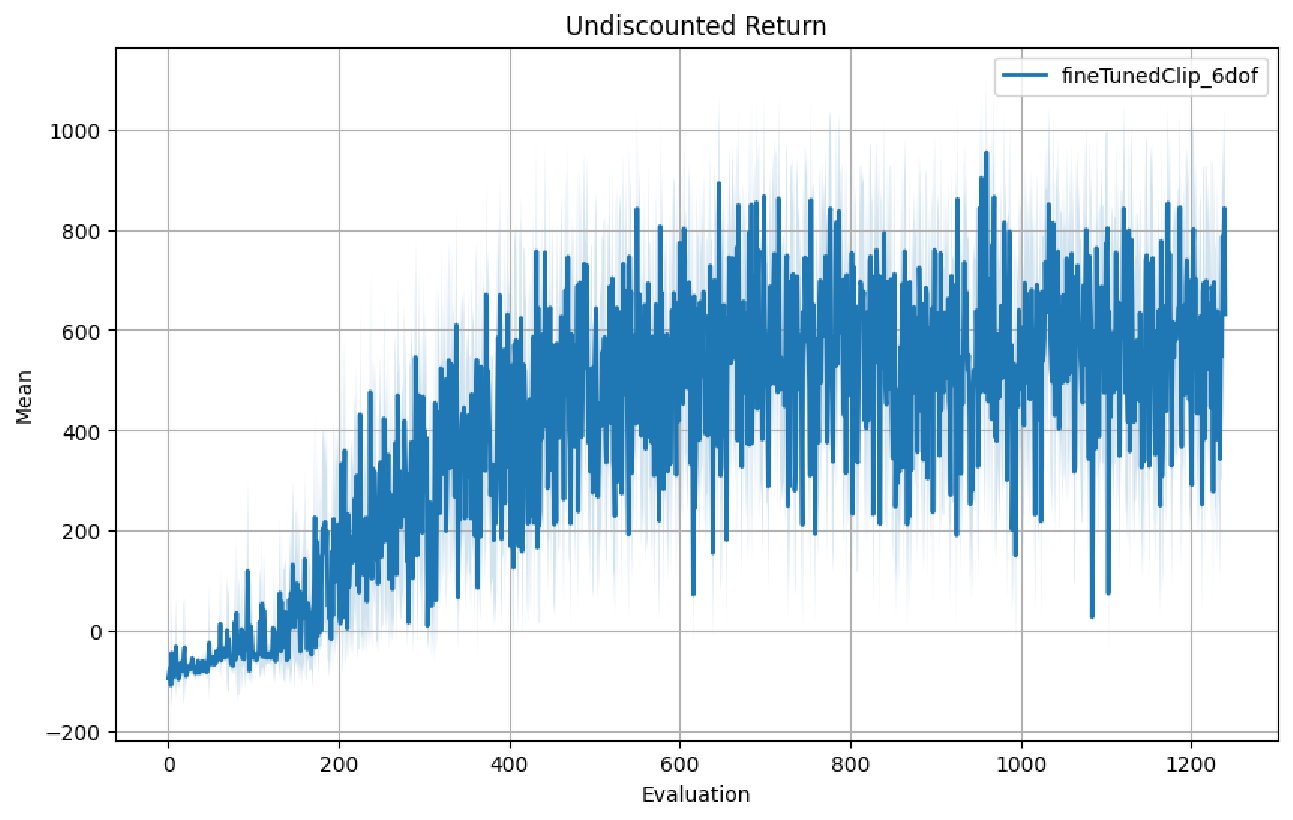
\includegraphics[width=0.8\textwidth]{Images/undiscounted_return.pdf}
    \caption[Undiscounted return.]{This figure represents the undiscounted mean return computed using the target policy of the agent.
    Each evaluation is performed every 20000 environment steps over 20 episodes.}
    \label{fig:undiscounted_return}
\end{figure}

This new hit agent achieved on a local evaluation without noise a 58 \% success rate over 100 episodes with a mean undiscounted return of 652, 
demonstrating an improvement over the previous rule-based hit policy.

\subsection{Improving the Switcher}
Other than replacing the rule based hit policy, a new home policy was implemented based on a PD controller:

\begin{equation*}
    \ddot{q} = K_p \cdot \left(q_{home} - q\right) - K_d \cdot \left(\dot{q}\right)
\end{equation*}
with $q_{home}$ equal to the desired position,  to return to and $K_p = 10$ and $K_d = 1$. These values were found by hand.

The switcher is a non differentiable policy that depends on a parameter vector $\theta$. It can be optimized with PGPE \cite{PGPE} and find an optimal set of parameters.
The reward function is a simple sparse reward:

\begin{equation*}
    r = \left\{
        \begin{aligned}
            1000 \quad &if \text{ our agent scores a goal} \\
            333 \quad &if \text{ the opponent gets a fault} \\
            -1000 \quad &if \text{ the opponent scores a goal} \\
            -333 \quad &if \text{ our agent gets a fault}
        \end{aligned}
    \right.
\end{equation*}

In this training environment episodes last 3000 steps and the discount rate $\gamma$ is set to 0.999.
The opponent used in this environment is still the baseline provided by the competition's organizers.
A plot of the mean return of the parameters distribution is illustrated in Figure \ref{fig:pgpe_return}.

\begin{figure}
    \centering
    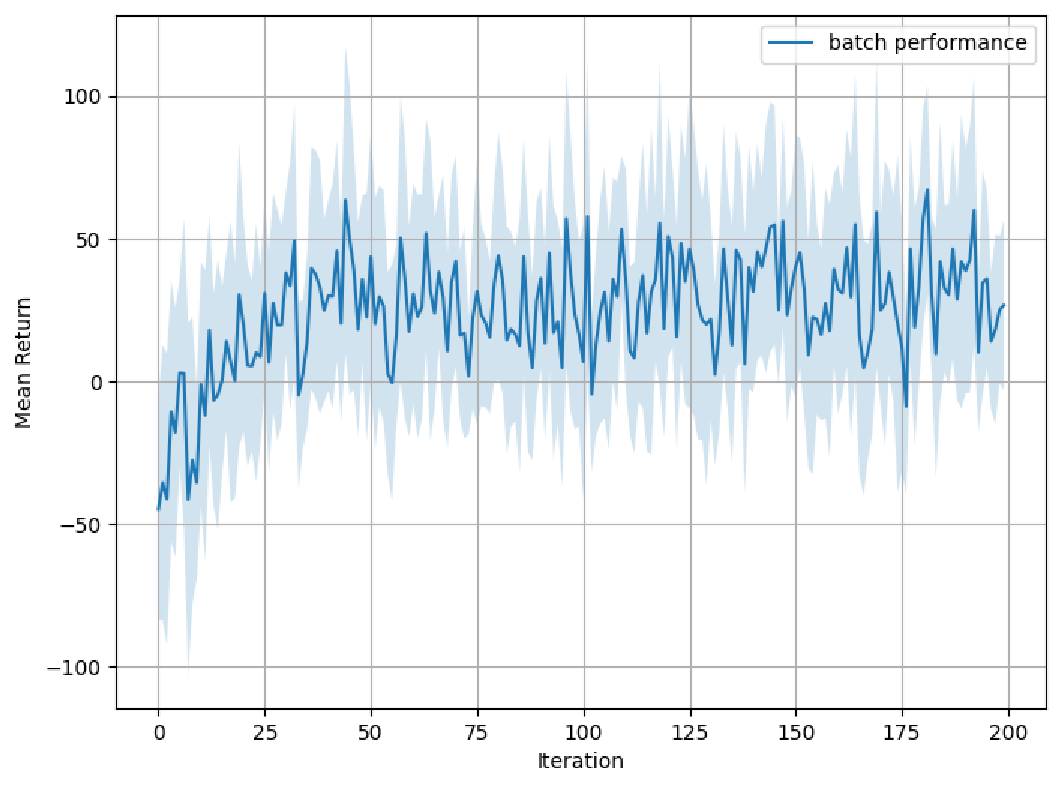
\includegraphics[width=0.7\textwidth]{Images/pgpe_return.pdf}
    \caption[PGPE mean return.]{In this figure each point correspond to the mean return obtained from a distribution $\rho$ of parameters. The return during training increases
    over zero, meaning that the hierarchical agent is consistently winning}
    \label{fig:pgpe_return}
\end{figure}